\documentclass{sbthesis} % source: Dr. Keith Schubert
%\usepackage[pdftex]{graphicx}
\usepackage{graphicx}
\usepackage{verbatim}
\usepackage{textcomp}
\usepackage{setspace}
\usepackage{float}
\usepackage{url}
\usepackage{regexpatch}% http://ctan.org/pkg/regexpatch
\usepackage[titletoc]{APPENDIX}
\usepackage{listings}

%%%%%%%%%%%%%%%%%%%%%%%%%%%%%%%%%%%%%%%%%%%%%%%%%%%%%%%%%%%%%%%%%%%%%%
%
% NOTE: I didn't have to do this.  Maybe it's because I'm using Miktex.  -- David Turner
%
% Note: bibtex omits page number from first page of bibliography, 
% which is not acceptable under CSUSB rules.  The following
% command can be used to fix the problem.  For this to work,
% you need to insert \FixBib after the first line in the bbl file 
% that bibtex generates.  Do this each time the bibliography
% changes.
%
% Source: http://www.cs.ubc.ca/~murphyk/Teaching/latex_tips.txt
%
%%%%%%%%%%%%%%%%%%%%%%%%%%%%%%%%%%%%%%%%%%%%%%%%%%%%%%%%%%%%%%%%%%%%%%
\newcommand{\FixBib}{%    PUT \FixBib in file.bbl after first line
    \setlength{\parsep}{\parskip}%
    \setlength{\itemsep}{0cm}%
    \setlength{\topsep}{\parskip}%
    \setlength{\parskip}{0cm}%
    \setlength{\partopsep}{0cm}%
    \setlength{\listparindent}{\parindent}%
    \setlength{\labelwidth}{10pt}%
    \setlength{\labelsep}{0pt}%
    \setlength{\leftskip}{0pt}%
    \setlength{\leftmargin}{0pt}%
}

\title{GRADEBADGE}
\TitleLineTwo{Development of a Cloud-Based Reward Application}
\author{Erwin Toni Soekianto}
\Department
\EmailAddress{soekiane@coyote.csusb.edu}
\Advisor{David Turner}
\Committee{Richard J. Botting}{Arturo I. Concepcion}
\CSUSBDate{June 2013}


\AbstractText{
The purpose of this project is to investigate the use of cloud-based services to deliver cutting-edge applications. For this purpose, a prototype of a reward application using badges, called GradeBadge, was developed to illustrate and explore this emerging paradigm. The cloud services utilized by this application include Heroku (for the application server), MongoLab (for the database), and Facebook (for authentication and social network integration).  The application server is written in Javascript and runs inside a Nodejs execution environment. The application is accessed through a Web browser running on either desktop or mobile computers.

On the client side, this application makes use of numerous Web technologies, including HTML5, CSS, Bootstrap, and Jquery. The project also made use of the Git version control system to manage source code and deployment of the application server to Heroku. The source code repository was stored remotely through the cloud-based service called GitHub. 

The purpose of the GradeBadge application is to help organizations interact with and motivate their members in a fun way. It keeps the members engaged by giving badges as rewards for their efforts or achievements. In order to facilitate adoption among users, GradeBadge is integrated with the social networking site Facebook.
}

\AcknowledgementText{
I would like to thank all the people with whom I have worked while pursuing my master's degree at California State University, San Bernardino (CSUSB). Studying in the School of Computer Science and Engineering at CSUSB has been a great learning experience.  I would like to thank the faculty of the School of Computer Science and Engineering who supported this project by serving on my committee: Dr. David Turner, Dr. Arturo Concepcion and Dr. Richard Botting.
}

\begin{document}
\Project  % defined in sbthesis.cls 

\Chapter{Introduction}

\section{Background}

A long time ago, businesses used to produce their own electric power. And due to engineering breakthrough in electric generator and transmission method, it became easier to produce and transmit electricity, to supply businesses that once produced their own electricity. As more businesses started buying electric power, making utility expanded and electricity cheaper. 

And today, just like the utilities, instead of buying servers to run your websites or applications, you rent servers or server spaces from cloud computing providers. Just like renting an apartment, even you are in the same building with other people, you still have your own space. As more people rent and buy computing power, making clould computing expanded and very popular. 

Today there are many cloud computing providers and they are providing different type of services. Some may provide hosting, database, code repositories or storage or combinations. Few famous providers are Google App Engine, Windows Azure, Amazon Web Services and Heroku. 

Google App Engine provides infrastructure to build the web application on the same scalable systems that power Google applications which support Phyton, Java, PHP and Go programming language. Google App Engine also provides several options for storing data, using App Engine Datastore, Google Cloud SQL, and Google Could Storage. Windows Azure provides similar service as Google App Engine but supports different set of programming language, such as .Net, Java, Node.js and Phyton.

Amazon provides scalable cloud computing, which allow users to choose what type of operating system and configuration of the servers they need, but it can scale as needed. It is more flexible to use any technologies, but require a lot of time and expertise to set it up. 

In this project, Heroku is used to as cloup application platform which support Node.js, Ruby, Clojure, Java, Phyton and Scala. Heroku lets you use and publish an application that people can use right away with no cost and obligation, and you can take advantage of the same scalable technologies that Facebook applications are built on, and the reliability, performance and security.

Among all the programming language supported in Heroku, in this project, Node.js is used as main programming language in the server side. HTML5, Javascript, Jquery and Bootstap framework will be used in the client side. As data store provider, MongoLab is used which support MongoDB database. 

Node.js and MongoDB in Heroku are often used together for scalable web technology. The following describe the clould computing service providers used in this project.

\section{Facebook}
Facebook is a very popular socila networking website and has billions of users. It has proven to be good platrom to use for web application and take advantage of its social networking, to connect to other Facebook users. Facebook also allows other application to access the user's data with their authorization using its API. \cite{Facebook}

\section{Heroku}
Cloud computing is a model which makes use of computer hardware and software that are accessed through the Internet as services. There are several choices of cloud computing services available, but for this project we choose the one provided by Heroku, the cloud computing partner of Facebook. \cite{Heroku}.

The reasons are that Heroku lets you use and publish an application that people can use right away with no cost and obligation, and you can take advantage of the same scalable technologies that Facebook applications are built on, and attain a similar level of reliability, performance and security. 

\section{MongoDB}
There are many different types of cloud-based datastore services to choose from. For this project we will use MongoDB, as it works well Node.js and Heroku. MongoDB is a scalable, high-performance, open source, NoSQL document-based database. MongoDB features include document-oriented storage, indexes, replication, high availability, auto-sharding, and querying. \cite{mongodb}

\section{MongoLab}
MongoLab is the cloud computing provider for MongoDB database, easily integrated with Heroku. \cite{mongolab}

\section{Git}
Git is a distributed version control system.  This project uses git with GitHub, a cloud-based provider of remote git repository storage.  Heroku uses git as a means to deploy web applications to its servers. Git allows easy creation of testing, staging, and production versions of the application. \cite{github}

\section{Bootstrap}
Bootstrap by Twitter provides responsive design framework that work well for application to be used in desktop, tablet and mobile phone. The UI of this project use Bootstrap. \cite{bootstrap}  

\section{Jquery}
Jquery is used for AJAX and DOM manipulation. \cite{JQuery}

\section{Node.js}
Cloud-based services support apps written in several different programming languages, such as Java, Python, PHP, Javascript, Ruby and many more. For this project we would use Javascript running in a Node.js context. Node.js is a platform built on Chrome's JavaScript runtime for easily building fast, scalable network applications. Node.js uses an event-driven, non-blocking I/O model that makes it lightweight and efficient, perfect for data-intensive real-time applications that run across distributed devices. \cite{nodejs}

\section{Purpose}
To explore the new technologies, to create cross-platform reward application that individual can use.

\section{Project Scope}
Project does not include database sharding features to allow greater degree of scalability. 

The GradeBadge application provides the following functionalities:
\begin{itemize}
\item Create group
\item Create Badge 
\item Add Member
\item Issue Badges to Members
\item View Badge Earned
\item Share Badge to Social Networking 
\end{itemize}

\section{Related Work}
There is another similar project in cloud computing, it used Google App Engine instead of Heroku as cloud computing providers, the main programming language used is Java with Google data store instead of Node.js and MongoDB. It uses Jquery Mobile as UI framework instead of BootStrap.   \cite{Manoj}
So there has been some increasing interest in cloud computing technology, and there are dozens other famous application that use similar technologies.  


\section{Project Limitations}
Users must have Facebook account,  logged in to facebook and authorized access to basic information (name, profile picture and friend list) .For best experience must use modern browser in either PC or tablet or smart phone.    

\section{Definitions, Acronyms, and Abbreviations}

The definitions, acronyms, and abbreviations used in the document are described in this section.

\begin{itemize}
\item GradeBadge: The name of this project
\item API: Application Programming Interface is a set of routines that an application uses to request and carry out low-level services performed by a computer's operating system; also, a set of calling conventions in programming that defines how a service is invoked through the application \cite{API}.
\item Cloud computing: Cloud computing is the use of computing resources (hardware and software) that are delivered as a service over a network (typically the Internet) \cite{cloudcomputing}.
\item JQuery: A javascript library provided by JQuery for building web based applications \cite{JQuery}.
\item UI: User Interface
\item CSUSB: California State University, San Bernardino.
\item HTML: HyperText Markup Language is the authoring language used to create documents on the World Wide Web \cite{w3}.
\item HTTPS: Hyper Text Transfer Protocol Secure is a secure network protocol used to encrypt data transferred  between server and client \cite{https}.
\item MVC\label{def:mvc}: Model-View-Controller is an architectural pattern used in software engineering to isolate business logic from user interface considerations \cite{MVC}.
\item UML: The Unified Modeling Language is the industry-standard language for specifying, visualizing, constructing, and documenting the artifacts of software systems \cite{uml}.
\item Microsoft Azure: Cloud Computing platform provided by Microsoft \cite{MicrosoftAzure}.
\item Google App Engine: Cloud Computing platform provided by Google 
\item Amazon Web Services: Cloud Computing platform provided by Amazon \cite{AWS}.
\item Heroku:Cloud Application platform provided by Heroku \cite{Heroku}.
\item Android : Mobile Operating System provided by Google \cite{Android}.
\item IOS : Mobile Operating System provided by Apple \cite{IOS}.
\item NoSQL: Uses key-value pairs for storing data unlike traditional Relational Database Management \cite{NoSql}.
\item JSON : Javascript Object Notation built using key and value pairs \cite{json}.
\item Ajax:  Asynchronous JavaScript and XML/JSON format for communicating from client to the server \cite{Ajax}.
\item OOP : Object Oriented Programming concept with objects representing real world entities. Methods expose state of the object \cite{OOP}.
\end{itemize}



\Chapter{Software Requirements Specification}

\section{External Interfaces Requirement}

\subsection{Hardware Interfaces}

The application is hosted in the Heroku application cloud service. The Web server communicates over HTTPS to ensure that data transferred between client and server is untampered and private. The system is a Web based application; users are required to use a high-speed Internet connection and use an up-to-date Web browser.

\subsection{Software Interfaces}

Javascript will be implemented throughout the Website in order to display the correct feature the user requested. And HTML5 may be implemented throughout the website in order to display the correct feature the user requested.

\subsection{Communication Interfaces}

This application is designed to be viewed on any Internet Web browser provided that Javascript and image features are enabled and the browser is HTML5 compatible. Performance may vary slightly between browsers; however, the functionality of the site should not be impaired.

In order to access this application, internet connection is required. On tablets or smart phones, when internet connection is not available, this application can be accessed through 3G, 4G or LTE networks.

\section{Functional Requirement}

The functions specified in this section directly correspond to work that will be conducted in this project as shown in the use case diagram in Figure ~\ref{fig:use_case}. 

\vspace{3em}
\begin{figure}[H]
\begin{center}
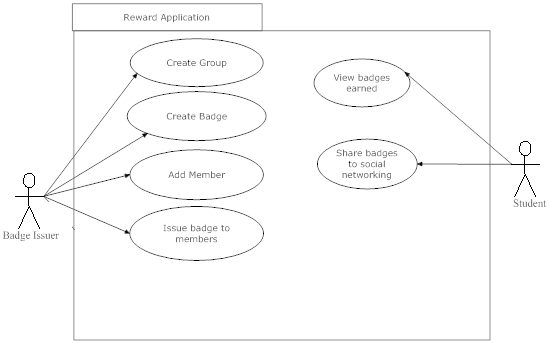
\includegraphics[height=3.8in,width=6.5in]{images/UseCase.png}
\caption{Use Case Diagram}
\label{fig:use_case}
\end{center}
\end{figure}

\subsection{Create Group}

This functionality allows organizers or badge issuers to create groups, which will have a set badge collection.

\subsection{Create Badge} 

This functionality allows badge issuers to create badge to be added to badge collection. A badge would have at least badge name and description.

\subsection{Add Member}

This functionality would allow organizers or badge issuers to add members into the groups as badge recipients. Member would have at least email address and name.

\subsection{Issue Badges to Members}

This functionality would allow badge issuers to issue badges to members. 

\subsection{View Badge Earned}

This functionality would allow badge recipients to view all the badges that they have earned.

\subsection{Share Badge to Social Networking} 

This functionality would allow badge recipients to share the badge to their social networking site such as Facebook

\section{Performance Requirement}

This application is going to be hosted in the Heroku cloud server, so the performance of this application would be high.
 
\section{Design Constraint}

This application requires internet-enabled devices and internet connection to perform. And every user must have Facebook account to be able to use this. 

\section{Software System Attributes}

The author will maintain the proper commenting and documentation throughout the duration of the project, following Google Javascript style guide \cite{googleguide}. 

\Chapter{System Architecture}

\section{Overview}
There are three main server entities in this applicatio, which are Heroku, Facebook, and MongoLab. When the client browser, either from desktop computer or tablet or smart phone, runs the application, it will hit the Heroku server, then the Heroku server will connect to Facebook server to check user authentication. And if the user is not logged-in, the user will be prompted with the Facebook login screen and submit the login data to Facebook server. 

After the user is authenticated to use the application, the application server will connect to MongoLab server to read and write the data. The application server may occasionally go to Facebook server to check the users' friend list or  post to user's wall or check whether the user is still logged-in. 

This application uses HTTPS exclusively for security reasons, except in the local developer environment, where we use unencrypted HTTP,  as shown in Figure ~\ref{fig:deployment}.

\vspace{3em}
\begin{figure}[H]
\begin{center}
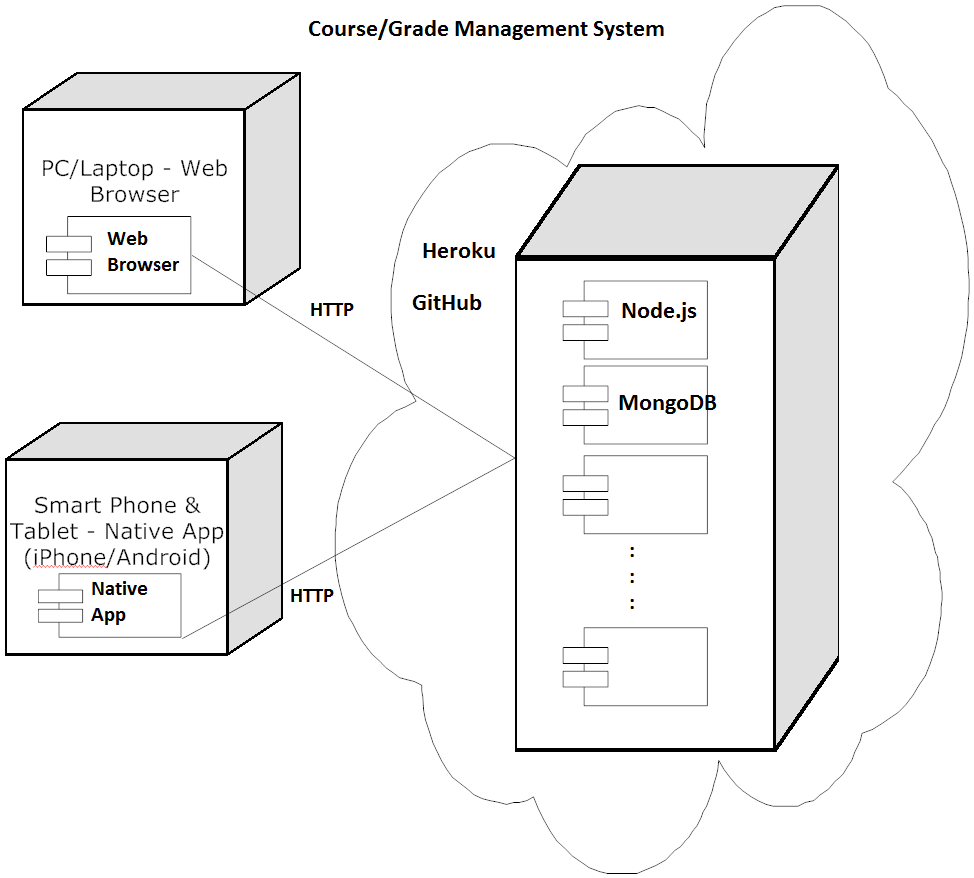
\includegraphics[height=3.8in,width=6.5in]{images/deployment.png}
\caption{Deployment Diagram}
\label{fig:deployment}
\end{center}
\end{figure}


\section{Deployment Workflow}
There are three type of environments used in the deployment workflow: development, staging and production.

Developers work on new features or bug fixes in development branches then only minor updates are committed directly to the stable development branch. Once the features are implemented and/or set of bugs are fixed, they are merged in to staging branch and deployed to staging environment for testing and quality assurance. After testing is completed, the snapshop of staging branch is kept for production deployment, otherwise the process will repeat until the testing is completed. On the release date, the working staging branch is deployed to production environment. 

Figure ~\ref{fig:system-integration} illustrates the deployment workflow.

\vspace{3em}
\begin{figure}[H]
\begin{center}
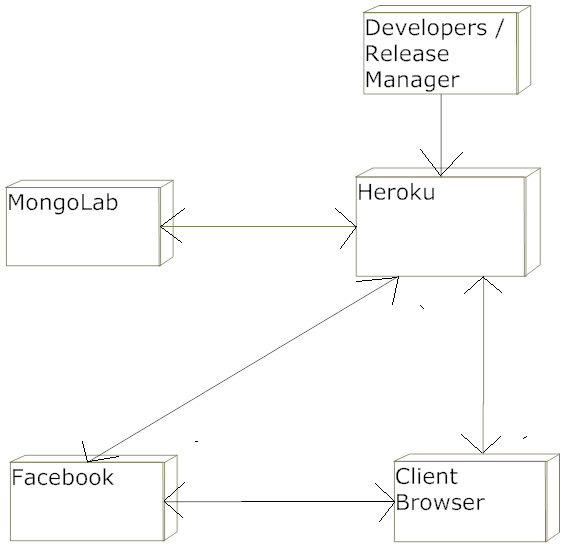
\includegraphics[height=3.8in,width=6.5in]{images/systemIntegration.png}
\caption{System Integration}
\label{fig:system-integration}
\end{center}
\end{figure}


On this project, git is used as code repositories, to manage developments, staging and production branch. And Heroku toolbelt is also used to set the enviroment config variable for each deployment. Heroku allows users to use git to deploy automatically from local repositories. 
 
\subsection{Developers/Release Manager}
In this project, developers first do unit testing in their local machines, then after the system reaches a certain point, the developer himself or assigned release manager will use git to push the changes to staging or production repositories that are connected to respective Heroku servers. 

Below are the commands the developer/release manager uses to start the application in the staging enviroment.
\begin{lstlisting}
$ foreman start
18:43:16 web.1  : started with pid 5540
18:43:16 web.1  : listening on 5000
\end{lstlisting}

Below are the commands for developer/release manager commits changes to master branch of the local repository, then followed by a push to master branch of the remote repository.
\begin{lstlisting}
$ git status
$ git add .
$ git commit -m "message here"
$ git push origin master
\end{lstlisting}

Below are the commands for developer/release manager uses to push to staging environment.
\begin{lstlisting}
$ git push staging master
\end{lstlisting}


\subsection{Heroku}
In this project there are two sets of heroku instances used: staging and production. 
The application running in Heroku connects to a database server running inside MongoLab using the MongoDB protocol to read and/or write data to database.  Heroku also talks to Facebook servers via Facebook's Open Graph API.

Below is the sample command in Heroku to create staging environment
\begin{lstlisting}
$ heroku create --remote staging
\end{lstlisting}

Below are the sample commands in Heroku to add environmetal variables in remote environment
\begin{lstlisting}
$ heroku config:set S3_KEY=XXX --remote staging
$ heroku config:set S3_SECRET=YYY --remote staging
\end{lstlisting}

\subsection{MongoLab}
In this project there are three sets of mongo databases used: development, staging and production. It is important to keep the versions of databases since new versions of changes may include changes in database structure, so rolling back or forward the application version would not cause any error. 

Below is the command on how to connect to remote Mongo Database that is hosted in MongoLab

\begin{lstlisting}
$ mongo <servername>.mongolab.com:<portno>/<dbname> 
   -u <dbuser> -p <dbpassword>
\end{lstlisting}

\subsection{Facebook}
Facebook is playing an important role in this project. Facebook provides user authentication and social media integration. Facebook allows connection using the Facebook API and Open Graph API.

\subsection{Client Browser}
Client browser uses HTTPS GET for static content, and HTTPS POST for AJAX request to Heroku. And client browser also connects to Facebook server directly using Facebook API and Open Graph API in HTTPS.
 

\Chapter{System Design}

\section{Design Overview}
GradeBadge application uses a client-server architecture model, and it uses MVC (Model View Controller) architecute in the client and server side. And all incoming AJAX requests are submitted using HTTP POST and contain data encoded using JSON.    

\section{Model View Controller Architecture}
This application is based on Model View Controller (MVC) Architecture. Model View Controller (MVC) architecture is a software design pattern for separating different components of a software application \cite{MVC}. There are three main categories in the MVC architecture:

\begin{itemize}
\item Model : it represents data in the application. All the business rules are handled in the model.
\item View: it represents UI components in the application. The UI components are responsible for presenting the model and for collecting user inputs.
\item Controller: it is responsible for updating the data in the model and notifying the view about changes in the model.
\end{itemize}

\section{Server-side Architecture Design}

All Nodejs modules that start with req{\_}*.js are request handler that get requested from router.js. All ajax requests will go through req{\_}op.js, that verifies the user logged-in to Facebook and app{\_}version is current. Every req{\_}op.js request must contains Facebook access{\_}token and app{\_}version. If the user is not logged-in to Facebook, req{\_}op.js returns the following JSON document, {login:true}, if the version is not current, then req{\_}op.js return the following JSON document, {ver:true}. 

\begin{itemize}
\item .env : This is the setup file that contains environment variables. This file only exist in developer local environment, and these values in this file would be set in each Heroku environment config for staging and production.  
\item .gitignore: This is the setup file that contains list of files or folders that will be ignored when committing or pushing to git repositories. 
\item .slugignore: This is the setup file that contains list of files or folders that will be ignored when calculating the slug limit in Heroku
\item package.json: This is the setup file that contains of list of dependencies and engine version use in the application. This file also contains application name, version and description.
\item Procfile: This is the setup file that tells Heroku how to launch the application
\item main.js: This is the main module in node js, which contains the code that verify all neccessary environment variables are set correctly. It also invoke initialization in neccesarry modules to start the application, after the initialization is completed, it starts the HTTP request handling loop. 
\item router.js: This module routes incoming requests to the right module.
\item app{\_}ajax.js: This module contains the application wide AJAX handling routines
\item app{\_}http.js: This module contains all of HTTP protocol routines for the application, caching headers, compression header and other HTTP based optimization are implemented in this module.
\item fb.js: This module contains all code that interact with Facebook.
\item logger.js: This module contains application wide logging functionalities.
\item model.js: This module initializes the database connnection pool during server start 
\item req{\_}app.js: This module handles request for application HTML template for badge earner
\item req{\_}counter.js: This module handles request for logging counter 
\item req{\_}file.js: This module handles request for static content.
\item req{\_}issuer.js: This module handles request for application HTML template for badge issuers
\item req{\_}mem.js: This module handles request for memory usage
\item req{\_}root.js: This module handles request for static content under the root URL
\item req{\_}op.js : This module handles all AJAX request from client and routes to appropriate modules.  
\end{itemize}

\section{Mapping of Model Classes to MongoDB}
There will be one node js module to represent the mongoDB collection, named model{\_}(collection{\_}name).js. And many-to-many relationships are represented by linking documents, named (a){\_}(b){\_}links

\begin{itemize}
\item model{\_}group.js: this node.js module represents Groups collection
\item model{\_}badge.js: this node.js module represents Badges colletion
\item model{\_}user.js: this node.js module represents Users collection
\item model{\_}group{\_}admin.js: this node.js module represents group{\_}admin{\_}links collection
\item model{\_}group{\_}member.js: this node.js module represents group{\_}member{\_}links collection
\item model{\_}user{\_}badge.js: this node.js module represents user{\_}badge{\_}links collection
\item model{\_}group{\_}badge.js: this node.js module represents group{\_}badge{\_}links collection
\end{itemize}

\section{Request Handler Operation}
There will be one node js module to handle ajax request from client, named op{\_}(request).js. Every request may read, write or update to and from more than one collection

\begin{itemize}
\item op{\_}read{\_}badges{\_}by{\_}group.js: this operation is for request for all badges in the given group
\item op{\_}read{\_}groups{\_}by{\_}admin.js: this operation is for request for all groups in the given admin
\item op{\_}save{\_}badge.js: this operation is for request for saving given badge details
\item op{\_}save{\_}group.js: this operation is for request for saving given group details
\end{itemize}

\section{Client-side Architecutre Design}


\begin{itemize}
\item app.html : This is the html template for badge earner page
\item issuer.html : This is the html template for badge issuer page
\item public{\_}root/channel.html : This is the static content required by Facebook 
\item public{\_}root/favicon.ico : This is the statuc content for icon use in the browser
\item public{\_}ver/app.js : This is the client java-script  
\item public{\_}ver/style.css: This is the css file use
\end{itemize}




\Chapter{Database Design}

\section{MongoDB}
 MongoDB is a scalable, high-performance, open source, NoSQL document-based database. MongoDB features include document-oriented storage, indexes, replication, high availability, auto-sharding, and querying.  \cite{mongodb}

\section{MongoLab}
MongoLab is the cloud computing provider for MongoDB database, easily integrated with Heroku. \cite{mongolab}

\section{Documents}
Data in MongoDB is stored in documents, and every document must have a primary key named {\_id}. Like reqular SQL-based database, documents are like row in a table, where in MongoDB, documents have flexible schema, but every document must have {\_id} field, even if you don't speficy the {\_id} field, mongoDB will add that automatically.  \cite{mongodb}

Although document structure is not enforced in MongoDB, different data model and structure may have significant impacts on MongoDB and application performace. So it is good to keep some kind of structure or pattern in data model.  

\section{Collections}
Documents in MongoDB are organized in collection, and basic database operations are performed based on collection. Indexes can be assigned in any field or subfield contained in documents within a MongoDB collection, and they are defined on per-collection level.  \cite{mongodb}   

\section{Data Model}
In this project, there are three main collections, User, Group and Badge Colletion. And there are four linkings colletions to represent the many-to-many relationship between the main collections.

\begin{itemize}
\item user : this collection contains the user information
\item group : this collection contains the group information  
\item badge : this collection contains the badge information
\item group{\_}admin{\_}links : this linking collection contains group{\_}id and user{\_}id, which represent the admin of a group
\item group{\_}member{\_}links : this linking collection contains group{\_}id and user{\_}id, which represent the member of a group
\item badge{\_}user{\_}links : this linking colletion contains badge{\_}id and user{\_}id, which reperesnt badges that user earned
\item group{\_}badge{\_}links : think linking collection contains group{\_}id and badge{\_}id, which represent badges that belong to a group
\end{itemize}





\Chapter{Project Implementation}

The GradeBadge application is designed to work on mobile, tablet devices and desktop computers. The UI of the application is developed using Bootstrap. When a page requires the data to be loaded from server or modified or deleted, a request is sent to the Web server over  HTTPS. The requests are sent to the Web server using Ajax. For handling Ajax requests and responses, this application uses JQuery Ajax API. All UI components are dynamically created or initialized in response to the data received from the Web server.

\newpage
\section{Loading Screen}
When the GradeBoard application is loaded, a loading screen is presented to the user as shown in the Figure ~\ref{fig:loading_screen}. The loading screen shows application logo and loading progess bar, and the screen is automatically redirected after the loading completed. 

\vspace{3em}
\begin{figure}[H]
\begin{center}
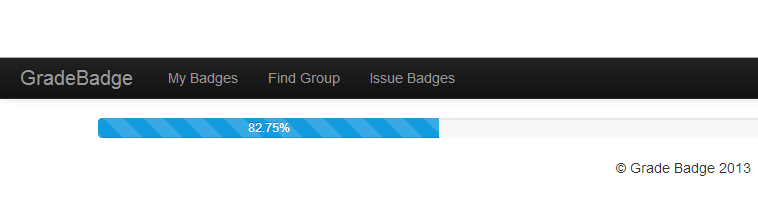
\includegraphics[height=3.8in,width=5.5in]{images/loading-screen.jpg}
\caption{GradeBadge Loading Screen}
\label{fig:loading_screen}
\end{center}
\end{figure}

\newpage
\section{Login Screen}
GradeBadge uses Facebook account for users to login. When the user is not logged-in to Facebook, the screen is automatically redirected to the Facebook login screen as shown in Figure~\ref{fig:login_screen}. Every user in the system can be badge issuer and badge earner.

\vspace{3em}
\begin{figure}[H]
\begin{center}
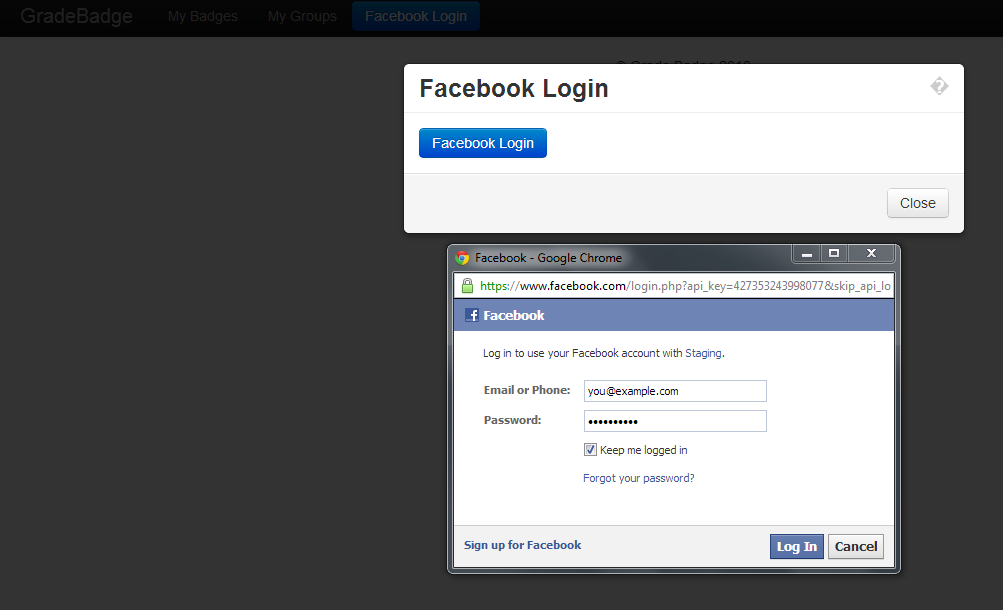
\includegraphics[height=3.3in,width=5.5in]{images/facebook-login.jpg}
\caption{GradeBadge Login Screen}
\label{fig:login_screen}
\end{center}
\end{figure}

\vspace{3em}
\begin{figure}[H]
\begin{center}
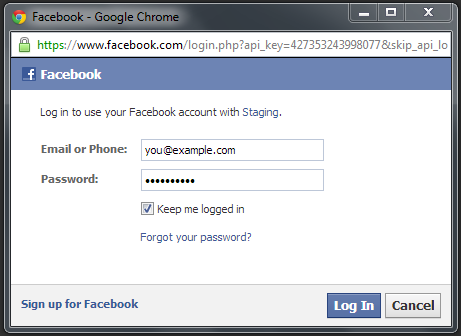
\includegraphics[height=3.8in,width=3.5in]{images/facebook-login1.jpg}
\caption{Facebook Login Screen}
\label{fig:fb_login_screen}
\end{center}
\end{figure}

\newpage
\section{Group Page}
 Badge issuers have access to list of groups that they manage as shown in Figure~\ref{fig:group-page1}. 

\vspace{3em}
\begin{figure}[H]
\begin{center}

\includegraphics[height=3.1in,width=5.5in]{images/group-page1.png}
\caption{GradeBadge Group Page}
\label{fig:group-page1}
\end{center}
\end{figure}

\newpage
\section{Add New Group Page}
Badge issuers can add new group by clicking at "Add New Group" button in group page, then the pop-up modal window to create new group will appear  as shown in Figure~\ref{fig:add-new-group}. 

\vspace{3em}
\begin{figure}[H]
\begin{center}
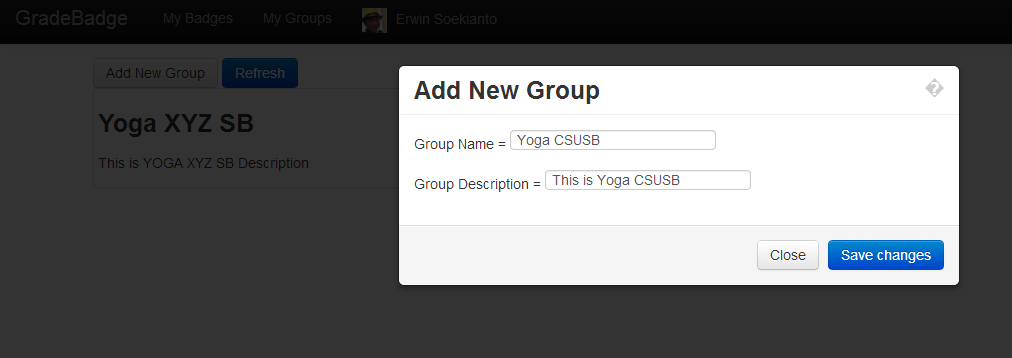
\includegraphics[height=3.1in,width=5.5in]{images/add-new-group.png}
\caption{GradeBadge Add New Group Page}
\label{fig:add-new-group}
\end{center}
\end{figure}

\newpage
\section{Group Page}
New groups have been added to group page as shown in Figure~\ref{fig:group-page2}. 

\vspace{3em}
\begin{figure}[H]
\begin{center}
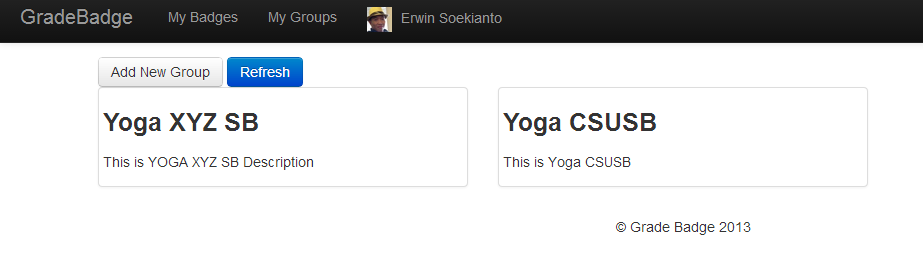
\includegraphics[height=6.1in,width=5.5in]{images/group-page2.png}
\caption{GradeBadge Group Page Added}
\label{fig:group-page2}
\end{center}
\end{figure}

\newpage
\section{Group Badge Page}
Badge issuers have access to list badges in a group by clicking at "Badge" button in a group thumbnail, then the application will display the list of badges in the selected group  as shown in Figure~\ref{fig:group-badge}. 

\vspace{3em}
\begin{figure}[H]
\begin{center}
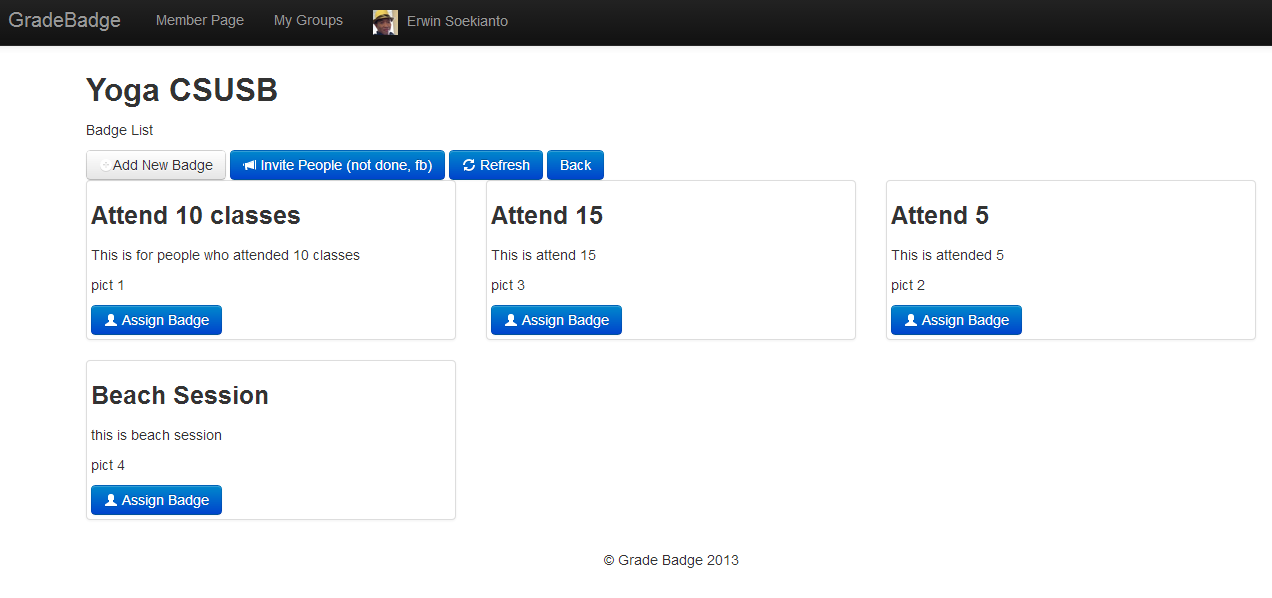
\includegraphics[height=5.1in,width=5.5in]{images/badge-page.png}
\caption{GradeBadge Group Badge Page}
\label{fig:group-badge}
\end{center}
\end{figure}

\newpage
\section{Add New Badge Page}
Badge issuers can add new badge by clicking at "Add New Badge" button in badge page, then the pop-up modal window to create new badge will appear  as shown in Figure~\ref{fig:add-new-badge}. 

\vspace{3em}
\begin{figure}[H]
\begin{center}
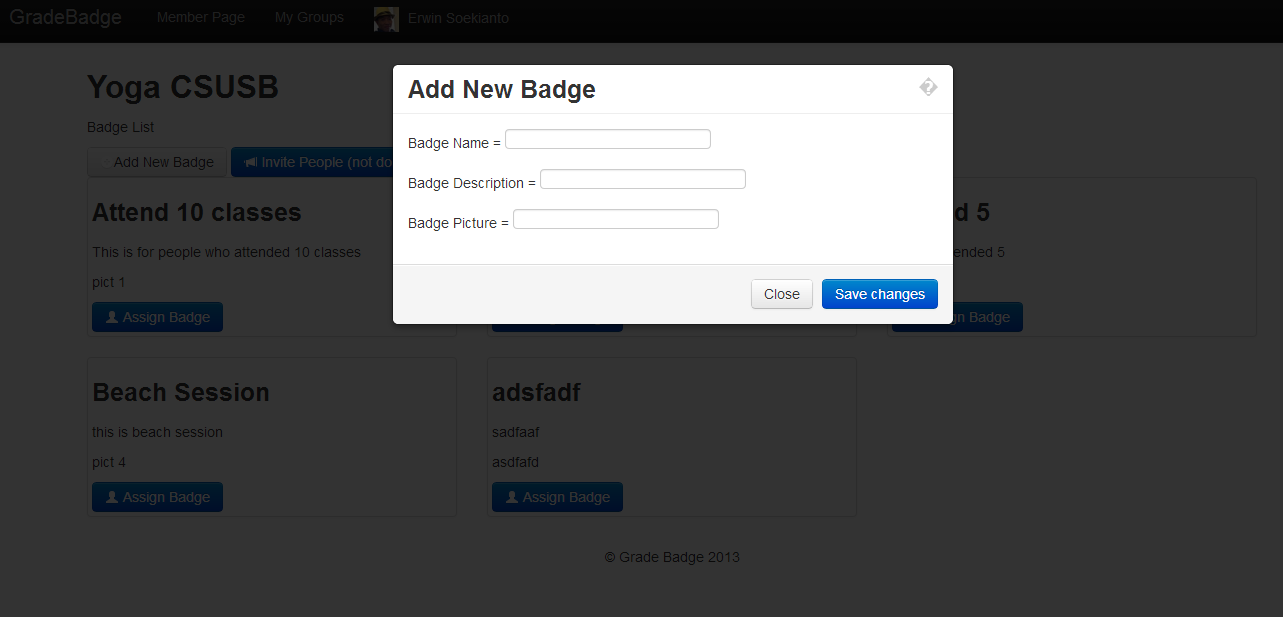
\includegraphics[height=5.1in,width=5.5in]{images/add-new-badge.png}
\caption{GradeBadge Add New Badge Page}
\label{fig:add-new-badge}
\end{center}
\end{figure}

\newpage
\section{Logging Counters Page}
The application also keeps track of errors, warnings and number of times a function is being callled. It can be accessed through web page as shown in Figure~\ref{fig:counters}. 

\vspace{3em}
\begin{figure}[H]
\begin{center}
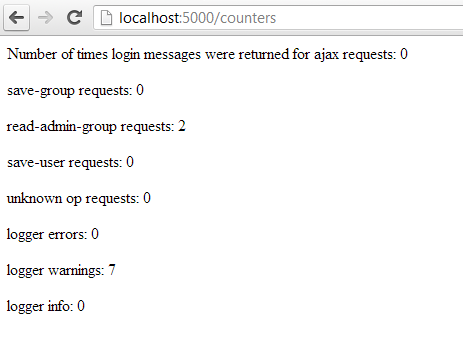
\includegraphics[height=3.1in,width=3.5in]{images/counters.png}
\caption{GradeBadge Logging Counters Page}
\label{fig:counters}
\end{center}
\end{figure}

\newpage
\section{Memory Statistic Page}
The application also monitors the memory and bandwidth usage of the application server. It can be accessed through web page as shown in Figure~\ref{fig:mem}. 

\vspace{3em}
\begin{figure}[H]
\begin{center}
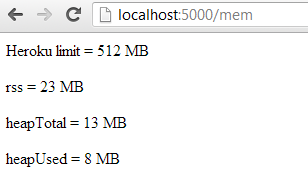
\includegraphics[height=3.1in,width=3.5in]{images/mem.png}
\caption{GradeBadge Memory Statistic Page}
\label{fig:mem}
\end{center}
\end{figure}




\Chapter{Conclusion and Future Direction}

\section{Conclusion}

GradeBadge is a cloud-based Web application that is hosted in Heroku, uses Nodejs and MongoDB, and that uses a responsive Web page design that works well inside browsers in desktop, tablet and smart phone computers. GradeBadge enables users to login with their Facebook account to simplify authentication and provide social networking features such as wall posting of badges earned and friend badge information. 

Cloud computing provides significant cost savings to developers when building applications that can be scaled up or down almost instantly to accomodate rapidly changing demand.

\section{Future Direction}

The GradeBadge application can be used as a sample to showcase the development of cloud-based cross-platform applications. This application can also be extended and enhanced in the future as follows. 

\begin{itemize}
\item Auto-sharding: Add auto-sharding to the Mongo database in order to support greater scalability. 
\item Other social networking: Implement authentication and integration with other social networking applications such as Twitter, Tumblr, Google+,  etc. 
\item Native App: Develop native versions of the application for iOS, Android and Windows Mobile.
\item API: Develop an API to enable other applications to integrate a reward system module into their applications.
\end{itemize}

%\Appendix{SERVER SOURCE CODE}
\small
\lstset{basicstyle=\ttfamily,breaklines=true}
\begin{lstlisting}
//main.js

\end{lstlisting}


%\Appendix{Model Classes Source Code Examples}
\small
\lstset{basicstyle=\ttfamily,breaklines=true}
\begin{lstlisting}
// model_group.js
var assert = require('assert');
var model = require('./model');

exports.create = function(group, cb) {
  model.db.collection('groups').insert(
    group,
    function(err) {
      model.db.close();
      if (err) return cb(err); 
      cb();
    }
  );  
};

exports.getByIds = function(group_ids, cb){
  model.db.collection('groups').find({'_id' : {$in: group_ids} }).toArray(function(err, groups){
    model.db.close();
    if (err) return cb(err);
    console.log('model_group getByIds groups array = '+ JSON.stringify(groups));  
    cb(groups);
  });
};

exports.getAll = function(cb){
  model.db.collection('groups').find().toArray(function(err, groups){
    model.db.close();
    if (err) return cb(err);
    console.log('model_group getByIds groups array = '+ JSON.stringify(groups));  
    cb(groups);
  });
};

exports.readGroupMembers = function(group, cb) {
  model.db.collection('group_member_links',{'uid' : true}).find(group).toArray(function(err, group_member_links){
    if (err) {model.db.close(); return cb(err);}
    console.log('model_group readGroupMembers group_member_links = '+ JSON.stringify(group_member_links));
    
    var member_ids = group_member_links.map(function(group_member_link) {return group_member_link.gid;});
    model.db.collection('users').find({'_id' : {$in: member_ids} }).toArray(function(err, members){
      model.db.close();
      if (err) return cb(err);
      console.log('model_group readGroupMembers members array = '+ JSON.stringify(members));  
      group.members = members;
      cb();
    });
    
  });    
};


\end{lstlisting}


%\chapter{APPENDIX A}


%\Appendix{Client Side Source Code}
\small
\lstset{basicstyle=\ttfamily,breaklines=true}
\begin{lstlisting}
//public_root\channel.html
<script src="//connect.facebook.net/en_US/all.js"></script>
\end{lstlisting}

\begin{lstlisting}
//public_ver\app.js
window.a = {};
a.creds = {};
a.m = {};
a.c = {};
a.v = {};

/* ------------------SCREENS---------------------- */
$(function() {
  var screens = {};
    
  (function (){
    Screen = function(name) {
      this.name = name;
      this.$mainDiv = $('#'+name);
    };
    
    Screen.prototype.transitionTo = function(speed, newScreen){
      this.$mainDiv.fadeOut(speed, function() {
        newScreen.$mainDiv.fadeIn(speed);
      });
    };    
    
    screens.loading     = new Screen('loading');
    screens.groups      = new Screen('groups');
    screens.title       = new Screen('title');
    screens.badges      = new Screen('badges');
    screens.myBadges    = new Screen('myBadges');
    screens.profile     = new Screen('profile'); 
    screens.login       = new Screen('login');
    screens.groupBadges = new Screen('groupBadges');
    screens.badgeMembers= new Screen('badgeMembers');
    screens.findGroups  = new Screen('findGroups');
  }());
  
  var currentScreen = screens.loading;
        
  a.screen = function(screenName, speed){
    if (speed === undefined) speed = 300;
    var newScreen = screens[screenName];
    if (newScreen.init) newScreen.init();
    currentScreen.transitionTo(speed, newScreen);
    currentScreen = newScreen;
  };
  
  a.refresh = function(){
    currentScreen.refresh();
  };

  a.rebuild = function(){
    currentScreen.rebuild();
  };
  
  screens.findGroups.rebuild = function(){
    $('#groups_list > li').remove();
    a.m.anyGroups.forEach(function(group, i){
        $('#groups_list').append(
          '<li class="span4">' +
            '<div class="thumbnail">' +
              '<h3>'+ group.name +'</h3>' +
              '<p>'+ group.desc +'</p>' +
              '<button id="group_edit" class="btn btn-primary" onclick="screens.findGroups.joinGroupBtn('+i+')" type="button">' +
                '<i class="icon-certificate icon-white"></i> Join</button>' +
            '</div>' +
          '</li>'
        );  
    });
  };
  
  screens.findGroups.joinGroupBtn = funtion(i){
    a.m.joinGroup(a.m.anyGroups[i]._id, function(){
      if (err) 
        alert('Err' + err.message);
      else
        a.screens('badges');
    });
  };
  
  screens.findGroups.refresh = function(){   
    a.m.readAnyGroups(function() {
      screens.findGroups.rebuild();
    });
  };
  
  screens.findGroups.init = function(){
    console.log('findGroups init');
    if (a.m.anyGroups === undefined) screens.findGroups.refresh();
  };
  
  screens.title.init = function(){
    FB.api('/me', function(response) {
      console.log('Screen init title');
      $('#name').html('<a href="#" onclick="a.screen(\'profile\')"><img width="25" height="25" style="margin-right:5" src="http://graph.facebook.com/' + response.id + '/picture" />  '+response.name+'</a>');
    });
  };
  
  screens.login.init = function(){
    screens.login.$mainDiv.html('<button class="btn btn-primary" type="button" onclick="a.fbLogin()">Facebook Login</button>');
    $('#loginModal').modal('show');
  };
  
  screens.groupBadges.init = function(){
    console.log('Curr Group = ' +JSON.stringify(a.v.currGroup));
    $('#groupname').html('<h2>'+ a.v.currGroup.name +'</h2>');
    if (a.v.currGroup.badges === undefined) screens.groupBadges.refresh();
  };
  
  screens.groupBadges.refresh = function(){   
    a.m.readGroupBadges(function() {
      screens.groupBadges.rebuild();
    });
  };
  
  screens.badgeMembers.init = function(){
    console.log('Curr Badge = ' +JSON.stringify(a.v.currBadge));
    $('#badgename').html('<h2>'+ a.v.currBadge.name +'</h2>');
    if (a.v.currBadge.members === undefined) screens.badgeMembers.refresh();
  };
  
  screens.badgeMembers.refresh = function(){   
    a.m.readBadgeMembers(function() {
      screens.badgeMembers.rebuild();
    });
  };
  
  screens.groups.refresh = function(){   
    a.m.readGroups(function() {
      screens.groups.rebuild();
    });
  };
  
  screens.badgeMembers.rebuild = function(){
    $('#badge_members_list > li').remove();
    a.v.currBadge.members.forEach(function(member, i){
        $('#badge_members_list').append(
          '<li class="span4">' +
            '<div class="thumbnail">' +
              '<h3>'+ member.name +'</h3>' +
              '<p>'+ member.uid +'</p>' +
              '<p>Status earned</p>' +
              '<p>photo, # badge earned</p>' +
              '<button id="group_edit" class="btn btn-primary" onclick="" type="button">' +
                '<i class="icon-certificate icon-white"></i> Assign (not done)</button>' +
            '</div>' +
          '</li>'
        );  
    });
  };
  
  screens.groupBadges.rebuild = function(){
    $('#group_badges_list > li').remove();
    a.v.currGroup.badges.forEach(function(badge, i){
        $('#group_badges_list').append(
          '<li class="span4">' +
            '<div class="thumbnail">' +
              '<h3>'+ badge.name +'</h3>' +
              '<p>'+ badge.desc +'</p>' +
              '<p>'+ badge.pict +'</p>' +
              '<button id="assign_badge" class="btn btn-primary" onclick="screens.groupBadges.selectBadgeBtn('+i+')" type="button">' +
                '<i class="icon-user icon-white"></i> Assign Badge</button>' + 
            '</div>' +
          '</li>'
        );  
    });
  };
  
  screens.groupBadges.selectBadgeBtn = function(i) {
    a.v.currBadge = a.v.currGroup.badges[i];
    screens.groupBadges.rebuild();
    a.screen('badgeMembers');
  };
  
  screens.groups.rebuild = function(){
    $('#groups_list > li').remove();
    a.m.groups.forEach(function(group, i){
        $('#groups_list').append(
          '<li class="span4">' +
            '<div class="thumbnail">' +
              '<h3>'+ group.name +'</h3>' +
              '<p>'+ group.desc +'</p>' +
              '<button id="group_edit" class="btn btn-primary" onclick="screens.groups.selectGroupBtn('+i+')" type="button">' +
                '<i class="icon-certificate icon-white"></i> Badges</button>' +
            '</div>' +
          '</li>'
        );  
    });
  };
  
  screens.groups.selectGroupBtn = function(i) {
    a.v.currGroup = a.m.groups[i];
    screens.groupBadges.rebuild();
    a.screen('groupBadges');
  };
  
  screens.groups.init = function(){
    if (a.m.groups === undefined) screens.groups.refresh();
  };
 
});
/*-----   END OF SCREENS ------------------ */

/*------------------ MODEL --------------------- */
a.m.readGroups = function(cb) { 
  $.ajax({
    url: '/op/read-groups-by-admin',
    type: 'post',
    dataType: 'json',
    cache: false,
    data: JSON.stringify( { 'accessToken': a.creds.accessToken } )
  })
  .done(function(data) {
    console.log('app.js data = '+ JSON.stringify(data));
    //if (data.login !== undefined) {
      //a.relogin(function() { $saveBtn.click(); });
    //} else 
    if (data.error !== undefined) {
      console.log('error = ' + data.error);
      cb(data.error);
    } else {
      console.log('group is read');
      a.m.groups = data.data;
      a.m.groups.sort(function(a,b) { return a.name < b.name ? -1 : 1});
      cb();
    }
  })
  .fail(function(jqxhr, textStatus, errorThrown) {
    if (errorThrown) console.log('Error: ' + errorThrown);
    else console.log('Error: ' + textStatus);
  });
}; 

a.m.readAnyGroups = function(cb) { 
  $.ajax({
    url: '/op/read-any-groups',
    type: 'post',
    dataType: 'json',
    cache: false,
    data: JSON.stringify( { 'accessToken': a.creds.accessToken } )
  })
  .done(function(data) {
    console.log('app.js data = '+ JSON.stringify(data));
    //if (data.login !== undefined) {
      //a.relogin(function() { $saveBtn.click(); });
    //} else 
    if (data.error !== undefined) {
      console.log('error = ' + data.error);
      cb(data.error);
    } else {
      console.log('group is read');
      a.m.anyGroups = data.data;
      a.m.anyGroups.sort(function(a,b) { return a.name < b.name ? -1 : 1});
      cb();
    }
  })
  .fail(function(jqxhr, textStatus, errorThrown) {
    if (errorThrown) console.log('Error: ' + errorThrown);
    else console.log('Error: ' + textStatus);
  });
}; 

a.m.joinGroup = function(gid, cb) { 
  $.ajax({
    url: '/op/join-group',
    type: 'post',
    dataType: 'json',
    cache: false,
    data: JSON.stringify( { 'accessToken': a.creds.accessToken, 'gid': gid } )
  })
  .done(function(data) {
    console.log('app.js data = '+ JSON.stringify(data));
    //if (data.login !== undefined) {
      //a.relogin(function() { $saveBtn.click(); });
    //} else 
    if (data.error !== undefined) {
      console.log('error = ' + data.error);
      cb(data.error);
    } else {
      console.log('group_member linked');
      cb();
    }
  })
  .fail(function(jqxhr, textStatus, errorThrown) {
    if (errorThrown) console.log('Error: ' + errorThrown);
    else console.log('Error: ' + textStatus);
  });
}; 

a.m.readGroupBadges = function(cb) { 
  $.ajax({
    url: '/op/read-badges-by-group',
    type: 'post',
    dataType: 'json',
    cache: false,
    data: JSON.stringify( { 'accessToken': a.creds.accessToken, 'gid' : a.v.currGroup._id } )
  })
  .done(function(data) {
    console.log('app.js data = '+ JSON.stringify(data));
    //if (data.login !== undefined) {
      //a.relogin(function() { $saveBtn.click(); });
    //} else 
    if (data.error !== undefined) {
      console.log('error = ' + data.error);
      cb(data.error);
    } else {
      console.log('badges are read');
      a.v.currGroup.badges = data.data;
      a.v.currGroup.badges.sort(function(a,b) { return a.name < b.name ? -1 : 1});
      cb();
    }
  })
  .fail(function(jqxhr, textStatus, errorThrown) {
    if (errorThrown) console.log('Error: ' + errorThrown);
    else console.log('Error: ' + textStatus);
  });
}; 

a.m.readBadgeMembers = function(cb) { 
  $.ajax({
    url: '/op/read-badge-members',
    type: 'post',
    dataType: 'json',
    cache: false,
    data: JSON.stringify( { 'accessToken': a.creds.accessToken, 'gid' : a.v.currGroup._id, 'bid' : a.v.currBadge._id } )
  })
  .done(function(data) {
    console.log('app.js data = '+ JSON.stringify(data));
    //if (data.login !== undefined) {
      //a.relogin(function() { $saveBtn.click(); });
    //} else 
    if (data.error !== undefined) {
      console.log('error = ' + data.error);
      cb(data.error);
    } else {
      console.log('members are read');
      a.v.currBadge.members = data.data;
      a.v.currBadge.members.sort(function(a,b) { return a.name < b.name ? -1 : 1});
      cb();
    }
  })
  .fail(function(jqxhr, textStatus, errorThrown) {
    if (errorThrown) console.log('Error: ' + errorThrown);
    else console.log('Error: ' + textStatus);
  });
}; 

/*----------- END OF MODEL ---------------- */

/*------------------- CONTROLER ---------------- */
a.c.saveNewGroup = function() { 
  //console.log(JSON.stringify( { 'name': $('#gname').val(), 'desc': $('#gdesc').val(), 'accessToken': a.creds.accessToken } ));
  $.ajax({
    url: '/op/save-group',
    type: 'post',
    dataType: 'json',
    cache: false,
    data: JSON.stringify( { 'name': $('#gname').val(), 'desc': $('#gdesc').val(), 'accessToken': a.creds.accessToken } )
  })
  .done(function(data) {
    console.log(JSON.stringify(data));
    
    if (data.login !== undefined) {
      a.fbRelogin(function() { $saveBtn.click(); });
    } else 
    if (data.error !== undefined) {
      console.log('error = ' + data.error);
      //$numDiv.html(data.error);
    }else{
      console.log('group is saved, id = ' + JSON.stringify(data.data));
      $('#addGroupModal').hide();
      //a.screen('groups');
      a.m.groups.push({'_id': data.data.gid, 'name': $('#gname').val(), 'desc': $('#gdesc').val() });
      a.rebuild();
    }
  })
  .fail(function(jqxhr, textStatus, errorThrown) {
    if (errorThrown) console.log('Error: ' + errorThrown);
    else console.log('Error: ' + textStatus);
  });
}; 

a.c.saveNewBadge = function() { 
  $.ajax({
    url: '/op/save-badge',
    type: 'post',
    dataType: 'json',
    cache: false,
    data: JSON.stringify( { 'name': $('#bname').val(), 'desc': $('#bdesc').val(), 'pict': $('#bpict').val(), 'gid': a.v.currGroup._id, 'accessToken': a.creds.accessToken } )
  })
  .done(function(data) {
    console.log(JSON.stringify(data));
    
    if (data.login !== undefined) {
      a.fbRelogin(function() { $saveBtn.click(); });
    } else if (data.error !== undefined) {
      console.log('error = ' + data.error);
      //$numDiv.html(data.error);
    }else{
      console.log('badge is saved, id = ' + JSON.stringify(data.data));
      $('#addBadgeModal').hide();
      a.screen('groupBadges');
      a.v.currGroup.badges.push({'_id': data.data.bid, 'name': $('#bname').val(), 'desc': $('#bdesc').val(), 'pict': $('#bpict').val(), 'gid': a.v.currGroup._id });
      a.rebuild();
    }
  })
  .fail(function(jqxhr, textStatus, errorThrown) {
    if (errorThrown) console.log('Error: ' + errorThrown);
    else console.log('Error: ' + textStatus);
  });
}; 


/* ----------------- END OF CONTROLLER ------------- */

/*------------------ VIEW ----------------- */
a.v.currGroup = null;


a.v.currBadge = null;

/* ----------------- END OF VIEW ------------- */


/* ----------------------------FB Business--------------------------------- */
a.fbRelogin = function(cb) {
console.log('a.relogin()');
  FB.getLoginStatus(function(response) {
    if (response.status === 'connected') {
      a.creds.uid = response.authResponse.userID;
      a.creds.accessToken = response.authResponse.accessToken;
      cb();
    } else if (response.status === 'not_authorized') {
      //a.screen.next('login');
    } else {
      //var $relogin = $('<button>Login to Facebook</button>');
      //$('.screen').hide();
      //$('body').append($relogin);
      //$relogin.click(function() {
      //  $relogin.remove();
      //  $('.screen').show();
      //  a.login(cb);
      }
  }); 
};

a.fbLogin = function(cb) {
  FB.login(function(response) {
    if (response.authResponse) {
      a.creds.uid = response.authResponse.userID;
      a.creds.accessToken = response.authResponse.accessToken;
      $('#loginModal').modal('hide');
      a.screen('title');
      //cb('');
    } else {
      a.screen('login');
      //cb('Login failed.');
    }
  });
};
    
a.fbInit = function (fbAppId) {
  FB.init({
    appId      : fbAppId,
    channelUrl : '://' + window.location.host + '/channel.html',
    status     : false,  // check the login status upon init?
    cookie     : false,  // set sessions cookies?
    xfbml      : false
  });
  FB.Canvas.setAutoGrow();
  FB.getLoginStatus(function(response) {
    if (response.status === 'connected') {
      a.creds.uid = response.authResponse.userID;
      a.creds.accessToken = response.authResponse.accessToken;
      a.screen('title');
    } else {
      a.screen('login');
    }
  });
};
  /* ------------------------------------------------------------- */
  
fbAsyncInit();
\end{lstlisting}



%\appendix  not used, from Dr. Schubert's template
\appendix
%\Appendix{SERVER SOURCE CODE}
\small
\lstset{basicstyle=\ttfamily,breaklines=true}
\begin{lstlisting}
//main.js

\end{lstlisting}


%\Appendix{Model Classes Source Code Examples}
\small
\lstset{basicstyle=\ttfamily,breaklines=true}
\begin{lstlisting}
// model_group.js
var assert = require('assert');
var model = require('./model');

exports.create = function(group, cb) {
  model.db.collection('groups').insert(
    group,
    function(err) {
      model.db.close();
      if (err) return cb(err); 
      cb();
    }
  );  
};

exports.getByIds = function(group_ids, cb){
  model.db.collection('groups').find({'_id' : {$in: group_ids} }).toArray(function(err, groups){
    model.db.close();
    if (err) return cb(err);
    console.log('model_group getByIds groups array = '+ JSON.stringify(groups));  
    cb(groups);
  });
};

exports.getAll = function(cb){
  model.db.collection('groups').find().toArray(function(err, groups){
    model.db.close();
    if (err) return cb(err);
    console.log('model_group getByIds groups array = '+ JSON.stringify(groups));  
    cb(groups);
  });
};

exports.readGroupMembers = function(group, cb) {
  model.db.collection('group_member_links',{'uid' : true}).find(group).toArray(function(err, group_member_links){
    if (err) {model.db.close(); return cb(err);}
    console.log('model_group readGroupMembers group_member_links = '+ JSON.stringify(group_member_links));
    
    var member_ids = group_member_links.map(function(group_member_link) {return group_member_link.gid;});
    model.db.collection('users').find({'_id' : {$in: member_ids} }).toArray(function(err, members){
      model.db.close();
      if (err) return cb(err);
      console.log('model_group readGroupMembers members array = '+ JSON.stringify(members));  
      group.members = members;
      cb();
    });
    
  });    
};


\end{lstlisting}


%\chapter{APPENDIX A}


%\Appendix{Client Side Source Code}
\small
\lstset{basicstyle=\ttfamily,breaklines=true}
\begin{lstlisting}
//public_root\channel.html
<script src="//connect.facebook.net/en_US/all.js"></script>
\end{lstlisting}

\begin{lstlisting}
//public_ver\app.js
window.a = {};
a.creds = {};
a.m = {};
a.c = {};
a.v = {};

/* ------------------SCREENS---------------------- */
$(function() {
  var screens = {};
    
  (function (){
    Screen = function(name) {
      this.name = name;
      this.$mainDiv = $('#'+name);
    };
    
    Screen.prototype.transitionTo = function(speed, newScreen){
      this.$mainDiv.fadeOut(speed, function() {
        newScreen.$mainDiv.fadeIn(speed);
      });
    };    
    
    screens.loading     = new Screen('loading');
    screens.groups      = new Screen('groups');
    screens.title       = new Screen('title');
    screens.badges      = new Screen('badges');
    screens.myBadges    = new Screen('myBadges');
    screens.profile     = new Screen('profile'); 
    screens.login       = new Screen('login');
    screens.groupBadges = new Screen('groupBadges');
    screens.badgeMembers= new Screen('badgeMembers');
    screens.findGroups  = new Screen('findGroups');
  }());
  
  var currentScreen = screens.loading;
        
  a.screen = function(screenName, speed){
    if (speed === undefined) speed = 300;
    var newScreen = screens[screenName];
    if (newScreen.init) newScreen.init();
    currentScreen.transitionTo(speed, newScreen);
    currentScreen = newScreen;
  };
  
  a.refresh = function(){
    currentScreen.refresh();
  };

  a.rebuild = function(){
    currentScreen.rebuild();
  };
  
  screens.findGroups.rebuild = function(){
    $('#groups_list > li').remove();
    a.m.anyGroups.forEach(function(group, i){
        $('#groups_list').append(
          '<li class="span4">' +
            '<div class="thumbnail">' +
              '<h3>'+ group.name +'</h3>' +
              '<p>'+ group.desc +'</p>' +
              '<button id="group_edit" class="btn btn-primary" onclick="screens.findGroups.joinGroupBtn('+i+')" type="button">' +
                '<i class="icon-certificate icon-white"></i> Join</button>' +
            '</div>' +
          '</li>'
        );  
    });
  };
  
  screens.findGroups.joinGroupBtn = funtion(i){
    a.m.joinGroup(a.m.anyGroups[i]._id, function(){
      if (err) 
        alert('Err' + err.message);
      else
        a.screens('badges');
    });
  };
  
  screens.findGroups.refresh = function(){   
    a.m.readAnyGroups(function() {
      screens.findGroups.rebuild();
    });
  };
  
  screens.findGroups.init = function(){
    console.log('findGroups init');
    if (a.m.anyGroups === undefined) screens.findGroups.refresh();
  };
  
  screens.title.init = function(){
    FB.api('/me', function(response) {
      console.log('Screen init title');
      $('#name').html('<a href="#" onclick="a.screen(\'profile\')"><img width="25" height="25" style="margin-right:5" src="http://graph.facebook.com/' + response.id + '/picture" />  '+response.name+'</a>');
    });
  };
  
  screens.login.init = function(){
    screens.login.$mainDiv.html('<button class="btn btn-primary" type="button" onclick="a.fbLogin()">Facebook Login</button>');
    $('#loginModal').modal('show');
  };
  
  screens.groupBadges.init = function(){
    console.log('Curr Group = ' +JSON.stringify(a.v.currGroup));
    $('#groupname').html('<h2>'+ a.v.currGroup.name +'</h2>');
    if (a.v.currGroup.badges === undefined) screens.groupBadges.refresh();
  };
  
  screens.groupBadges.refresh = function(){   
    a.m.readGroupBadges(function() {
      screens.groupBadges.rebuild();
    });
  };
  
  screens.badgeMembers.init = function(){
    console.log('Curr Badge = ' +JSON.stringify(a.v.currBadge));
    $('#badgename').html('<h2>'+ a.v.currBadge.name +'</h2>');
    if (a.v.currBadge.members === undefined) screens.badgeMembers.refresh();
  };
  
  screens.badgeMembers.refresh = function(){   
    a.m.readBadgeMembers(function() {
      screens.badgeMembers.rebuild();
    });
  };
  
  screens.groups.refresh = function(){   
    a.m.readGroups(function() {
      screens.groups.rebuild();
    });
  };
  
  screens.badgeMembers.rebuild = function(){
    $('#badge_members_list > li').remove();
    a.v.currBadge.members.forEach(function(member, i){
        $('#badge_members_list').append(
          '<li class="span4">' +
            '<div class="thumbnail">' +
              '<h3>'+ member.name +'</h3>' +
              '<p>'+ member.uid +'</p>' +
              '<p>Status earned</p>' +
              '<p>photo, # badge earned</p>' +
              '<button id="group_edit" class="btn btn-primary" onclick="" type="button">' +
                '<i class="icon-certificate icon-white"></i> Assign (not done)</button>' +
            '</div>' +
          '</li>'
        );  
    });
  };
  
  screens.groupBadges.rebuild = function(){
    $('#group_badges_list > li').remove();
    a.v.currGroup.badges.forEach(function(badge, i){
        $('#group_badges_list').append(
          '<li class="span4">' +
            '<div class="thumbnail">' +
              '<h3>'+ badge.name +'</h3>' +
              '<p>'+ badge.desc +'</p>' +
              '<p>'+ badge.pict +'</p>' +
              '<button id="assign_badge" class="btn btn-primary" onclick="screens.groupBadges.selectBadgeBtn('+i+')" type="button">' +
                '<i class="icon-user icon-white"></i> Assign Badge</button>' + 
            '</div>' +
          '</li>'
        );  
    });
  };
  
  screens.groupBadges.selectBadgeBtn = function(i) {
    a.v.currBadge = a.v.currGroup.badges[i];
    screens.groupBadges.rebuild();
    a.screen('badgeMembers');
  };
  
  screens.groups.rebuild = function(){
    $('#groups_list > li').remove();
    a.m.groups.forEach(function(group, i){
        $('#groups_list').append(
          '<li class="span4">' +
            '<div class="thumbnail">' +
              '<h3>'+ group.name +'</h3>' +
              '<p>'+ group.desc +'</p>' +
              '<button id="group_edit" class="btn btn-primary" onclick="screens.groups.selectGroupBtn('+i+')" type="button">' +
                '<i class="icon-certificate icon-white"></i> Badges</button>' +
            '</div>' +
          '</li>'
        );  
    });
  };
  
  screens.groups.selectGroupBtn = function(i) {
    a.v.currGroup = a.m.groups[i];
    screens.groupBadges.rebuild();
    a.screen('groupBadges');
  };
  
  screens.groups.init = function(){
    if (a.m.groups === undefined) screens.groups.refresh();
  };
 
});
/*-----   END OF SCREENS ------------------ */

/*------------------ MODEL --------------------- */
a.m.readGroups = function(cb) { 
  $.ajax({
    url: '/op/read-groups-by-admin',
    type: 'post',
    dataType: 'json',
    cache: false,
    data: JSON.stringify( { 'accessToken': a.creds.accessToken } )
  })
  .done(function(data) {
    console.log('app.js data = '+ JSON.stringify(data));
    //if (data.login !== undefined) {
      //a.relogin(function() { $saveBtn.click(); });
    //} else 
    if (data.error !== undefined) {
      console.log('error = ' + data.error);
      cb(data.error);
    } else {
      console.log('group is read');
      a.m.groups = data.data;
      a.m.groups.sort(function(a,b) { return a.name < b.name ? -1 : 1});
      cb();
    }
  })
  .fail(function(jqxhr, textStatus, errorThrown) {
    if (errorThrown) console.log('Error: ' + errorThrown);
    else console.log('Error: ' + textStatus);
  });
}; 

a.m.readAnyGroups = function(cb) { 
  $.ajax({
    url: '/op/read-any-groups',
    type: 'post',
    dataType: 'json',
    cache: false,
    data: JSON.stringify( { 'accessToken': a.creds.accessToken } )
  })
  .done(function(data) {
    console.log('app.js data = '+ JSON.stringify(data));
    //if (data.login !== undefined) {
      //a.relogin(function() { $saveBtn.click(); });
    //} else 
    if (data.error !== undefined) {
      console.log('error = ' + data.error);
      cb(data.error);
    } else {
      console.log('group is read');
      a.m.anyGroups = data.data;
      a.m.anyGroups.sort(function(a,b) { return a.name < b.name ? -1 : 1});
      cb();
    }
  })
  .fail(function(jqxhr, textStatus, errorThrown) {
    if (errorThrown) console.log('Error: ' + errorThrown);
    else console.log('Error: ' + textStatus);
  });
}; 

a.m.joinGroup = function(gid, cb) { 
  $.ajax({
    url: '/op/join-group',
    type: 'post',
    dataType: 'json',
    cache: false,
    data: JSON.stringify( { 'accessToken': a.creds.accessToken, 'gid': gid } )
  })
  .done(function(data) {
    console.log('app.js data = '+ JSON.stringify(data));
    //if (data.login !== undefined) {
      //a.relogin(function() { $saveBtn.click(); });
    //} else 
    if (data.error !== undefined) {
      console.log('error = ' + data.error);
      cb(data.error);
    } else {
      console.log('group_member linked');
      cb();
    }
  })
  .fail(function(jqxhr, textStatus, errorThrown) {
    if (errorThrown) console.log('Error: ' + errorThrown);
    else console.log('Error: ' + textStatus);
  });
}; 

a.m.readGroupBadges = function(cb) { 
  $.ajax({
    url: '/op/read-badges-by-group',
    type: 'post',
    dataType: 'json',
    cache: false,
    data: JSON.stringify( { 'accessToken': a.creds.accessToken, 'gid' : a.v.currGroup._id } )
  })
  .done(function(data) {
    console.log('app.js data = '+ JSON.stringify(data));
    //if (data.login !== undefined) {
      //a.relogin(function() { $saveBtn.click(); });
    //} else 
    if (data.error !== undefined) {
      console.log('error = ' + data.error);
      cb(data.error);
    } else {
      console.log('badges are read');
      a.v.currGroup.badges = data.data;
      a.v.currGroup.badges.sort(function(a,b) { return a.name < b.name ? -1 : 1});
      cb();
    }
  })
  .fail(function(jqxhr, textStatus, errorThrown) {
    if (errorThrown) console.log('Error: ' + errorThrown);
    else console.log('Error: ' + textStatus);
  });
}; 

a.m.readBadgeMembers = function(cb) { 
  $.ajax({
    url: '/op/read-badge-members',
    type: 'post',
    dataType: 'json',
    cache: false,
    data: JSON.stringify( { 'accessToken': a.creds.accessToken, 'gid' : a.v.currGroup._id, 'bid' : a.v.currBadge._id } )
  })
  .done(function(data) {
    console.log('app.js data = '+ JSON.stringify(data));
    //if (data.login !== undefined) {
      //a.relogin(function() { $saveBtn.click(); });
    //} else 
    if (data.error !== undefined) {
      console.log('error = ' + data.error);
      cb(data.error);
    } else {
      console.log('members are read');
      a.v.currBadge.members = data.data;
      a.v.currBadge.members.sort(function(a,b) { return a.name < b.name ? -1 : 1});
      cb();
    }
  })
  .fail(function(jqxhr, textStatus, errorThrown) {
    if (errorThrown) console.log('Error: ' + errorThrown);
    else console.log('Error: ' + textStatus);
  });
}; 

/*----------- END OF MODEL ---------------- */

/*------------------- CONTROLER ---------------- */
a.c.saveNewGroup = function() { 
  //console.log(JSON.stringify( { 'name': $('#gname').val(), 'desc': $('#gdesc').val(), 'accessToken': a.creds.accessToken } ));
  $.ajax({
    url: '/op/save-group',
    type: 'post',
    dataType: 'json',
    cache: false,
    data: JSON.stringify( { 'name': $('#gname').val(), 'desc': $('#gdesc').val(), 'accessToken': a.creds.accessToken } )
  })
  .done(function(data) {
    console.log(JSON.stringify(data));
    
    if (data.login !== undefined) {
      a.fbRelogin(function() { $saveBtn.click(); });
    } else 
    if (data.error !== undefined) {
      console.log('error = ' + data.error);
      //$numDiv.html(data.error);
    }else{
      console.log('group is saved, id = ' + JSON.stringify(data.data));
      $('#addGroupModal').hide();
      //a.screen('groups');
      a.m.groups.push({'_id': data.data.gid, 'name': $('#gname').val(), 'desc': $('#gdesc').val() });
      a.rebuild();
    }
  })
  .fail(function(jqxhr, textStatus, errorThrown) {
    if (errorThrown) console.log('Error: ' + errorThrown);
    else console.log('Error: ' + textStatus);
  });
}; 

a.c.saveNewBadge = function() { 
  $.ajax({
    url: '/op/save-badge',
    type: 'post',
    dataType: 'json',
    cache: false,
    data: JSON.stringify( { 'name': $('#bname').val(), 'desc': $('#bdesc').val(), 'pict': $('#bpict').val(), 'gid': a.v.currGroup._id, 'accessToken': a.creds.accessToken } )
  })
  .done(function(data) {
    console.log(JSON.stringify(data));
    
    if (data.login !== undefined) {
      a.fbRelogin(function() { $saveBtn.click(); });
    } else if (data.error !== undefined) {
      console.log('error = ' + data.error);
      //$numDiv.html(data.error);
    }else{
      console.log('badge is saved, id = ' + JSON.stringify(data.data));
      $('#addBadgeModal').hide();
      a.screen('groupBadges');
      a.v.currGroup.badges.push({'_id': data.data.bid, 'name': $('#bname').val(), 'desc': $('#bdesc').val(), 'pict': $('#bpict').val(), 'gid': a.v.currGroup._id });
      a.rebuild();
    }
  })
  .fail(function(jqxhr, textStatus, errorThrown) {
    if (errorThrown) console.log('Error: ' + errorThrown);
    else console.log('Error: ' + textStatus);
  });
}; 


/* ----------------- END OF CONTROLLER ------------- */

/*------------------ VIEW ----------------- */
a.v.currGroup = null;


a.v.currBadge = null;

/* ----------------- END OF VIEW ------------- */


/* ----------------------------FB Business--------------------------------- */
a.fbRelogin = function(cb) {
console.log('a.relogin()');
  FB.getLoginStatus(function(response) {
    if (response.status === 'connected') {
      a.creds.uid = response.authResponse.userID;
      a.creds.accessToken = response.authResponse.accessToken;
      cb();
    } else if (response.status === 'not_authorized') {
      //a.screen.next('login');
    } else {
      //var $relogin = $('<button>Login to Facebook</button>');
      //$('.screen').hide();
      //$('body').append($relogin);
      //$relogin.click(function() {
      //  $relogin.remove();
      //  $('.screen').show();
      //  a.login(cb);
      }
  }); 
};

a.fbLogin = function(cb) {
  FB.login(function(response) {
    if (response.authResponse) {
      a.creds.uid = response.authResponse.userID;
      a.creds.accessToken = response.authResponse.accessToken;
      $('#loginModal').modal('hide');
      a.screen('title');
      //cb('');
    } else {
      a.screen('login');
      //cb('Login failed.');
    }
  });
};
    
a.fbInit = function (fbAppId) {
  FB.init({
    appId      : fbAppId,
    channelUrl : '://' + window.location.host + '/channel.html',
    status     : false,  // check the login status upon init?
    cookie     : false,  // set sessions cookies?
    xfbml      : false
  });
  FB.Canvas.setAutoGrow();
  FB.getLoginStatus(function(response) {
    if (response.status === 'connected') {
      a.creds.uid = response.authResponse.userID;
      a.creds.accessToken = response.authResponse.accessToken;
      a.screen('title');
    } else {
      a.screen('login');
    }
  });
};
  /* ------------------------------------------------------------- */
  
fbAsyncInit();
\end{lstlisting}



\nocite{*}
\urlstyle{same}
\raggedright
\sloppy
%\renewcommand{\normalsize}{\fontsize{12pt}{12pt}\selectfont} 
\normalsize
\Bibliography{main}

\end{document}
